\section{Zero excess starts fix the total amount of executed work}\label{app:zero}
At a strict return let \(S\) contain the \(s\) completed votes, with winner \(a\). At the last dispatch the observed votes \(S_0\) formed a subset of \(S\). We construct an input compatible with \(S_0\) on which the serial run locks by index \(s\). Keep the observed votes of \(S_0\) in positions \(1,\ldots,s\), assign every other position of that prefix to \(a\), and honor all other known votes beyond \(s\). The resulting prefix's multiset can be formed from \(S\) by retaining the specified observations and replacing the remaining votes by \(a\). This cannot reduce \(a\)'s lead. The prefix therefore certifies \(a\) strictly. With \(B=0\), \(J\le s\) at the last dispatch. Since every completion has launched, \(s=J\). On the realized input, these \(J\) finished paths form a serial prefix. Its certificate implies \(K\le J\), and the allowance imposes \(J\le K\). If the service instead exhausts its quota without a strict certificate, a smaller locking prefix would also lock the full quota prefix, so \(K\ge Q\). These cases prove invariance of \(\sum_{i=1}^{\min(K,Q)}w_i\) under all compliant schedules, including when paths have schedule-dependent completion times through their common service clock.

\section{Occupancy majorization for an arbitrary slot count}\label{app:major}
At a reachable zero-overrun history let \(h(S)=|S|+m(S)\) where \(m(S)\) counts the fewest further completions that can produce a strict lock or exhaust the full \(N\)-vote panel. The absolute quota separately limits further work to \(Q-|S|\) completions. Filling \(m\) further outcomes with the current leader gives such a decision, so retaining observed indices in the first \(h\) positions and assigning its other positions to the leader constructs a compatible \(K\le h\). Thus \(M\le h\). On a zero-allowance history, all previously admitted indices are at most \(M\), by the monotonicity of \(M\). Conversely a compatible serial locking prefix of length \(M<N\) contains all observations and must include at least \(m\) additional positions. If \(M=N\), exhaustion gives the same inequality. Hence \(M=h\). The width permitted just after replenishment is \(\min(P,m(S),Q-|S|)\), a nonincreasing function of newly observed information since each vote decreases the remaining count by one and changes the margin by at most one.

In particular, $m=\min\{R,\max(0,\lfloor(R-g)/2\rfloor+1)\}$, where $R=N-|S|$ and $g=\gap(S)$. This includes the terminal boundary. The absolute quota and slot cap apply separately.

Fix votes and let $w'_i\le w_i$ for every job. Greedy on $w'$ starts and finishes each job no later in virtual time than any admissible comparator on $w$. Induct on the comparator's launches. Its previously completed paths started no later on the shortened greedy execution and needed weakly less work. Thus at the comparator's next launch the shortened greedy run includes all the observations used for admission, so it has already filled to at least the same cumulative frontier. If shortened greedy already terminated, the common prefix result shows that it already finished the same jobs. In particular, greedy on $w'$ includes all completions of greedy on $w$ at the same virtual time. The nonincreasing active-width cap derived above yields $h_{G,w'}(t)\le h_{G,w}(t)$, with both profiles set to zero after their respective decisions.

For a schedule $A$ of finite duration $D$, let $E$ be any union of intervals and fix $0<\epsilon<1$. Reparameterize its timeline by the strictly increasing map
\[
 \phi_\epsilon(t)=\int_0^t (\mathbf{1}_E(u)+\epsilon\mathbf{1}_{E^c}(u))\,du .
\]
Transform every start $s_i$ and finish $e_i$ and set $w'_i=\phi_\epsilon(e_i)-\phi_\epsilon(s_i)>0$ for its completed paths. Keep the work of unlaunched paths unchanged. Running the same jobs between transformed endpoints with unit virtual rate realizes that shorter input. All event orders, simultaneous returns, slot counts and vote histories at dispatches are preserved. Write $D_\epsilon=\phi_\epsilon(D)$. On this input greedy completes by $D_\epsilon$ and executes the same total work as the transformed schedule. Therefore
\[
 \int_E h_A+\epsilon\int_{[0,D]\setminus E}h_A
 =\sum_{i\le J}w'_i=\int_0^{D_\epsilon}h_{G,w'}(u)\,du
 \le \int_0^{D_\epsilon}h_{G,w}(u)\,du .
\]
The last profile is bounded by $P$ and independent of $\epsilon$. Letting $\epsilon$ decrease to zero proves \eqref{eq:major}, without introducing zero-work jobs. For $E=\{h_A>j\}$ subtract $j|E|$ from both sides and upper-bound the right side by $\int (h_{G,w}-j)_+$. Thus greedy maximizes this integral for every threshold. Put $\theta_j=2c_j-c_{j-1}-c_{j+1}$. The discrete identity $c_k=c_1k-\sum_{j=1}^{P-1}\theta_j(k-j)_+$, equal total work, and $\theta_j\ge0$ give $T_G\le T_A$.

For an ordered panel that must complete all $N$ paths, the same comparison follows with cumulative frontier $\min(N,|S|+P)$ and greedy width $\min(P,N-|S|)$. These two quantities are respectively nondecreasing and nonincreasing as completions arrive, and every scheduling policy executes exactly the same work. The shortened-input comparison and time compression therefore give \eqref{eq:major} and optimality under concave prices for this fixed-panel objective.

If $\theta_j<0$ for any $j<P$, take any even $N\ge\max(2j,P)$, all votes equal and quota $Q=j+1$. No set of $j$ votes certifies, allowing all $Q$ launches at the outset. Give the first $j-1$ jobs work two and the following two work one. Greedy takes $c_{j+1}+c_{j-1}$. A policy starting $j$ jobs and replenishing at the short job's finish takes $2c_j$. At $j=1$, $c_0=0$ accounts for the already completed greedy run. This establishes necessity. As a finite independent check, a dynamic program maximizing each threshold over every integer-time launch choice verified all 4,488 comparisons in 1,416 configurations at four through eight slots, representing 1,651,840 complete histories.

\subsection{Sharp price ratios for nonconcave clocks}\label{app:sharp}
Let $\gamma=\max_{1\le k\le P}\widehat c_k/c_k$. The upper bound in the main text holds on every panel, and when $\gamma=1$ it is exact. For $\gamma>1$, a maximizing $j$ lies strictly between two contact widths $0\le a<j<b\le P$ of the piecewise-linear concave majorant. The value $\widehat c_j$ is the height of their chord. Write $S=\mathrm{lcm}(b-a,j-a)$ and $L=S/(j-a)$. Choose a multiple $d$ of $P$ with $d>S+a+P$. Use $N=2(d+b-1)$ and $Q=d+a+S$. The first $d$ paths have work $\epsilon>0$ and vote A. The next $a$ have work $L$, the following $S$ have work one, and these $a+S$ paths all vote B. All remaining votes can be chosen arbitrarily.

Both schedules execute the first $d$ paths in full batches of $P$. After $s\le d-P$ prefix completions the admissible in-flight allowance before quota and slot caps is $d+b-s$, at least $P$. After all $d$ prefix votes arrive it is exactly $b$. Each suffix completion reduces the number of unresolved votes and the A lead by one. The inequality on $d$ keeps A ahead, so the vote constraint continues to allow $b$ in-flight requests throughout the suffix. Neither policy can certify early, and they finish all $Q$ paths. Greedy first starts all $a$ long jobs and fills the other $b-a$ slots with short jobs for $S/(b-a)$ virtual steps. It then runs only the long jobs until $L$. For $a=0$ the second segment costs zero because greedy is already done. Its suffix cost is
\[
 \frac{S}{b-a}c_b+\left(L-\frac{S}{b-a}\right)c_a
 = L\left(\frac{j-a}{b-a}c_b+\frac{b-j}{b-a}c_a\right)=L\widehat c_j .
\]
The comparator starts the long jobs and keeps only $j-a$ short jobs in flight until $L$, at cost $Lc_j$. The integrality of both short-job batch counts follows from the choice of $S$. The common prefix cost is $(d/P)c_P\epsilon$. Letting $\epsilon$ decrease to zero yields a greedy-to-comparator ratio approaching $\widehat c_j/c_j=\gamma$. Since $T_{\rm opt}\le T_A$, this establishes the matching lower bound on the supremum. The construction was also replayed with the indexed gate for all 210 triples $a<j<b$ at slot counts two through eight.

To see why repricing fixes the execution, set $N=8$, $Q=4$, $P=3$, $B=0$, with unit work on the first four paths and prices $(10,11,13)$. Four starts are safe even before any votes return. Run the first two together. Run the next two together if the first pair finishes in less than $11.25$ wall-time units, and serially otherwise. At the original prices the schedule costs $22$. Repricing that virtual trajectory under the concave majorant $(10,11.5,13)$ gives $23$. Executing the same wall-time rule anew at those prices instead gives $11.5+20=31.5$. The proof uses the repriced trajectory.

\section{Enumerating the certificate-work relaxation}
Use one bit per path among the first \(Q\). A terminal mask must be a strict certificate or the full exhausted quota. For any completed \(j\), discard a mask lacking an \(i<j\) with \(w_i\le w_j\). Also test the largest completed index \(j\): even if every other vote in the mask had already arrived, \eqref{eq:f} must have permitted the launch through \(j\). These necessary tests leave a superset of attainable masks. Compute the vector of lower bounds in \eqref{eq:lp} for each retained mask. Componentwise larger requirement vectors can be dropped when minimizing across masks.

The resulting LP has only \(P\) occupancy variables. Combine the \(m=1\) row with the virtual time requirement and use the total-work constraint for \(m=P\). Write the resulting requirement vector as \(b\). Its dual is
\[
 \max_{y\ge0} b^\top y
 \quad\text{subject to}\quad
 \sum_{m=1}^P\min(k,m)y_m\le c_k\quad(k=1,\dots,P).
\]
We enumerate its vertices with exact rational arithmetic, then choose the smallest optimum across the masks. Its cost grows exponentially with the absolute quota through the number of candidate terminal sets. The certificate calculation can run offline on traces and leaves the online index scan unchanged.

\paragraph{An independent check with continuous launch delays.}
For integer work there exists an optimal schedule which starts only at integer virtual times. To see this, fix the order of the starts and completions through termination, including inequalities that keep unfinished requests' natural end after the deciding event. Write \(s_i\) for job \(i\)'s start. Its natural completion is \(s_i+w_i\). All imposed event orders give difference inequalities with integer offsets between start variables. Remove zero-width idle periods and set \(s_1=0\). For a schedule no slower than \(G\), all starts can be bounded by \(\lceil T_G/\min_k c_k\rceil\). Inside this order region the objective sums linear differences between the event times at each width. The closure is a bounded difference-constraint polyhedron, whose vertices have integral coordinates: tight equalities determine the start variables by integer differences along an anchored forest. A linear objective attains its minimum at one of the vertices. When a vertex merges events, process simultaneous completions before launches. The observations contain all those required for the original dispatches. If a decision now occurs earlier, remove subsequent dispatches. This operation preserves feasibility and does not increase elapsed time. There are only finitely many event orders. This proves existence on the integer grid even when the original competitor may use a continuous timer.

We enumerated safe schedules by dynamic programming with independently enumerated unseen votes. Across 11,776 configurations with three or four paths, two or three slots, integer work in \(\{1,2\}\), multiple budget settings, and increasing, flat or nonmonotone width costs, all work bounds held. The lower bound matched the exact optimum in 9,390 configurations and improved on the virtual-time-only floor in 6,537. Waiting could beat greedy in 3,112. A second oracle admitting starts on a half-unit grid gave the same optima. A distinct test of the zero-allowance theorem included 17,640 panel settings and 70,560 affine-price comparisons. These checks serve as implementation audits in addition to the proofs.

\section{What can a timer guarantee?}\label{app:timer}
At a completion event, some combination of the active votes may be sufficient to decide. Waiting for the next completion protects those requests from additional interference. It can also delay a short decisive vote until a slow request returns. Take sixteen A votes with four slots, \(Q=14,B=1\), and works \((L,2,1,1,\ldots,1)\). By virtual time 3, eight A votes have returned and path 1 still runs. Path 10 may safely start. Greedy obtains the ninth vote and decides at time 4. A policy that postpones this last start until the next completion decides at \(L\). The ratio grows without bound.

\begin{theorem}[Bounded waiting]\label{th:wait}
If a safe policy \(D\) fills to the indexed frontier except during a finite union of withholding intervals of realized total virtual duration \(H\), and refills at their right endpoints, then \(V_G\le V_D\le V_G+H\). The upper bound is sharp with \(N=16,P=4,Q=14,B=1\).
\end{theorem}
\begin{proof}
Let \(I\) be the union of the withholding intervals and set \(C(t)=t-|I\cap[0,t]|\) on \(0\le t\le V_D\). If \(C(V_D)=V_D-H\le V_G\), then \(V_D\le V_G+H\) directly. To cover the remaining case, for any \(0\le u<C(V_D)\) define \(\phi(u)=\sup\{t\le V_D:C(t)\le u\}\). At a collapsed interval this chooses its right endpoint, when \(D\) refills if still running. We have \(u\le\phi(u)\le u+H\) and \(\phi(v)-\phi(u)\ge v-u\) for \(u\le v\). By induction, each launch made by \(G\) by \(u\) has occurred under \(D\) by \(\phi(u)\), unless \(D\) has returned. Indeed, previously launched paths that finished under \(G\) have received enough virtual time to finish under \(D\). Their votes allow the same cumulative launch count, and at \(\phi(u)\) policy \(D\) fills to its frontier. When \(V_G<C(V_D)\), take \(u=V_G\). Those observations give a lock or quota exhaustion, so \(V_D\le\phi(V_G)\le V_G+H\). The lower bound follows from virtual launch dominance up to return. In the preceding example a single wait for \(H<L-4\) delays the decision from 4 to \(4+H\).
\end{proof}
This bound limits extra virtual time. A change in active width also changes its wall-clock price. Appendix~\ref{app:clock} gives a physical upper bound in terms of \(H\) and the measured variation of adjacent prices.

\section{Interpreting a cap on waiting in wall time}\label{app:clock}
Let \(c_{\max}=\max_k c_k\), and let \(L_+=\max(0,\max_{k<P}(c_{k+1}-c_k))\) and \(L_-=\max(0,\max_{k<P}(c_k-c_{k+1}))\). For \(P=1\) set both variation terms to zero. Suppose the nonterminal schedule always keeps a path active. If \(J\) and \(C\) paths have launched and completed in greedy by its decision, then a scheduler that withholds legal starts for a union of virtual intervals of total duration \(H\) satisfies
\[
          T_D-T_G \le H\big(c_{\max}+ C L_+ + J L_-\big).
\]
The resulting wall bound permits either ordering of \(T_D\) and \(T_G\). Theorem~\ref{th:wait} follows on each realized sequence of adaptive postponements or private random draws.

Write \(J_A(t)\) and \(C_A(t)\) for launches and completions by virtual time \(t\), taking zero at negative times. On \(0\le t<V_G\), virtual-time dominance bounds the two counts for \(D\) above by those for \(G\). The compressed-clock proof also bounds them below by the corresponding counts for \(G\) at \(t-H\). Integrating the launch deficit therefore costs at most \(JH\): each launch contributes for at most \(H\) time units. The completion deficit similarly integrates to at most \(CH\). At each time occupancy is launched count minus completed count, so excess width under \(D\) is no larger than the completion deficit and its shortfall is no larger than the launch deficit. Bounding the resulting price changes by \(L_+\) and \(L_-\) gives at most \(H(CL_++JL_-)\) extra elapsed time up to \(V_G\). The remaining virtual tail has length at most \(H\) and price at most \(c_{\max}\). An independent small-panel check evaluated the virtual bound on 24,768 allowed schedules or schedule comparisons and attained its upper limit on 3,096.

\section{Clock envelopes at positive allowance}\label{app:box}
The certificate bound $L(c)$ is an infimum of linear functions of the price vector $c$ over a common set of occupancy vectors, so it is concave. For a question with several panels, sum these bounds and the corresponding greedy times to obtain a concave lower bound $L_q(c)$ and a positive linear denominator $G_q(c)$. For $c$ in a box, write $c=\sum_v\lambda_v v$ using its corners. The ratio $L_q(c)/G_q(c)$ is bounded below by a weighted average of $L_q(v)/G_q(v)$, with weights proportional to $\lambda_vG_q(v)$. Taking each question's worst corner and then averaging gives an upper bound on the question-mean saving for every shared fixed clock in the box. Four widths require sixteen corners. If the within-question prices vary while remaining inside the box, charge the certificate bound at the componentwise minima and greedy at the maxima. The calibration measures eight block averages at each width in one session. The resulting envelope is a conditional sensitivity calculation.

\section{Admission with partially indexed votes}\label{app:bag}
For a prospective launch $j$, the serial-relative promise rules out a decisive prefix before $j-B$. Test $t=\max(0,j-B-1)$ because a strict lock remains a lock after later votes arrive. At this prefix maximize the possible lead among all vote assignments consistent with the information exposed to the gate. The indexed rule fixes all observed indices in the prefix, and fills each missing position with a vote for their current leader. The unordered gate knows the mask of completed positions and the multiset of all returned votes but forgets their pairing. Enumerate which sub-multiset of returns could occupy the completed positions in the prefix, then fill the missing positions to maximize the lead. The prefix-plus-multiset gate further fixes the initial contiguous returned votes in their observed positions before performing this enumeration. A launch is safe if this maximum is at most $N-t$. Physical slots and the absolute quota apply to all three rules. The comparison concerns assignments compatible with a single snapshot. A gate that retains its earlier observations could infer additional associations. The fully indexed decision can maintain the cumulative tally through $t=\max(0,J-B)$ together with the number of completed positions in that prefix. Only the last $B$ launched positions can lie beyond $t$, so their individual returns suffice in addition to label totals and the engine's active-request ledger. When $J$ grows by one, at most one such record enters the cumulative tally. It uses the same fixed trajectories and terminal rule as the index-aware policy.

\section{Inputs, statistics and sources of variation}\label{app:data}
The AIME, AMC and GSM8K traces came from the public \href{https://huggingface.co/datasets/reasoning-cues/rollouts-qwen4b/tree/b8c33b85a1a6cdfb23b06a5f9d696f52950780e4}{Reasoning Cues Qwen3-4B-Base archive} at revision \texttt{b8c33b85}. For AIME the fixed within-question shuffle produced two disjoint sixteen-path panels per question. The AMC analysis used the second of two distinct draws for each question. For GSM8K the parser removed whitespace from the last balanced boxed answer and recorded missing or truncated answers as abstentions. Shard names matching the first-draw unsteered pattern were sorted by the SHA-256 digest of a fixed namespace followed by the published path. The parser, eight selected shard object IDs and protocol were frozen before fetching their contents. All 3,200 selected trajectories belonged to complete panels. No extra model calls were used to forecast future votes in this evaluation.

For each of the 200 GSM8K questions, the paired saving was one minus the indexed-to-comparator time ratio for the admission comparisons. For each interval we sampled 200 questions with replacement and took the 2.5\% and 97.5\% quantiles of the resulting question means. The prespecified comparisons used 10,000 resamples with seed 19431. The two retrospective comparisons against the unordered and prefix-plus-multiset gates used 20,000 resamples with seed 651. These intervals treat questions as exchangeable, conditional on the selected shards and generation seeds. Published trajectory text and indices do not supply a complete execution environment for reconstructing the original sampler. Generated work includes partial canceled paths. A path count, a generated-token count, an invoice and an entire question's response time are distinct resources.

All eight selected shards had positive mean indexed-versus-buffered savings. Leaving out each shard in turn gave a question-mean saving ranging from 8.15\% to 9.23\% at 3,968 tokens.

\begin{table}[htbp]\centering
\caption{GSM8K sensitivity to a fixed width clock, in question-mean percent time saved. References are the buffered gate in the first row and indexed greedy in the remaining rows.}\label{tab:sens}
\begin{tabular}{lrrr}\toprule
Policy & 512 & 2,048 & 3,968\\\midrule
Indexed versus buffered & 8.934 & 8.880 & 8.709\\
Repeated conditional wait & $-76.040$ & $-75.005$ & $-73.244$\\
First conditional wait, eight-step cap & $-0.307$ & $-0.302$ & $-0.300$\\
First eligible wait, eight-step cap & $-0.229$ & $-0.225$ & $-0.224$\\
Hindsight best single wait & 0.103 & 0.100 & 0.115\\\bottomrule
\end{tabular}
\end{table}

The best-single-wait enumeration includes every eligible event on greedy's path because no prior launch differs before a first deviation. This enumeration excludes schedules which intentionally postpone more than once or which choose arbitrary continuous delays. Its optimum is directly realizable with future information, whereas the certificate-work relaxation bounds a larger action class without requiring its optimizer to correspond to a real schedule.

\section{Paired output-limit experiment on the A800}\label{app:cap}
The 32 eligible question hashes and the order of the four runs per question were fixed before the first model output. We used a separate seed namespace for this study and took every path from the same 1,024-token reference per question. The two policies returned identical answers within each cap. Across caps, the answer changed on two questions. Each question contributed one timed pair at each cap within a single device session. At 384 tokens 15 questions saved wall time and 17 took longer. At 1,024 tokens 22 saved time and 10 took longer. The paired estimates in the main text average individual question ratios. The summed costs below also include work already performed by paths canceled at return.

\begin{table}[htbp]\centering
\caption{Absolute cost of running each fixed-work policy on all 32 questions. Correct and certified count question-level decisions. Request starts and generated tokens include canceled requests. References for the paired savings are the buffered row at the same cap.}\label{tab:abscap}
\small\begin{tabular}{rlrrrrrr}\toprule
Cap & Gate & Wall time (s) & Steps & Generated tokens & Starts & Correct & Certified\\\midrule
384 & Indexed & 153.33 & 26,895 & 95,159 & 384 & 26 & 26\\
384 & Buffered & 154.77 & 27,159 & 95,303 & 384 & 26 & 26\\
1,024 & Indexed & 158.22 & 27,578 & 96,855 & 380 & 27 & 27\\
1,024 & Buffered & 161.02 & 27,834 & 96,611 & 380 & 27 & 27\\\bottomrule
\end{tabular}\end{table}
Both gates took longer in absolute time at the larger output limit. A change in relative saving compares indexed with buffered at each cap and allows their absolute times to increase. Including the 32 full references, the 160 timed panels generated 515,582 tokens in 835.24 seconds of synchronized panel time. The full 16-vote plurality answered 27 of the 32 questions correctly under each cap.

\begin{figure}[htbp]\centering
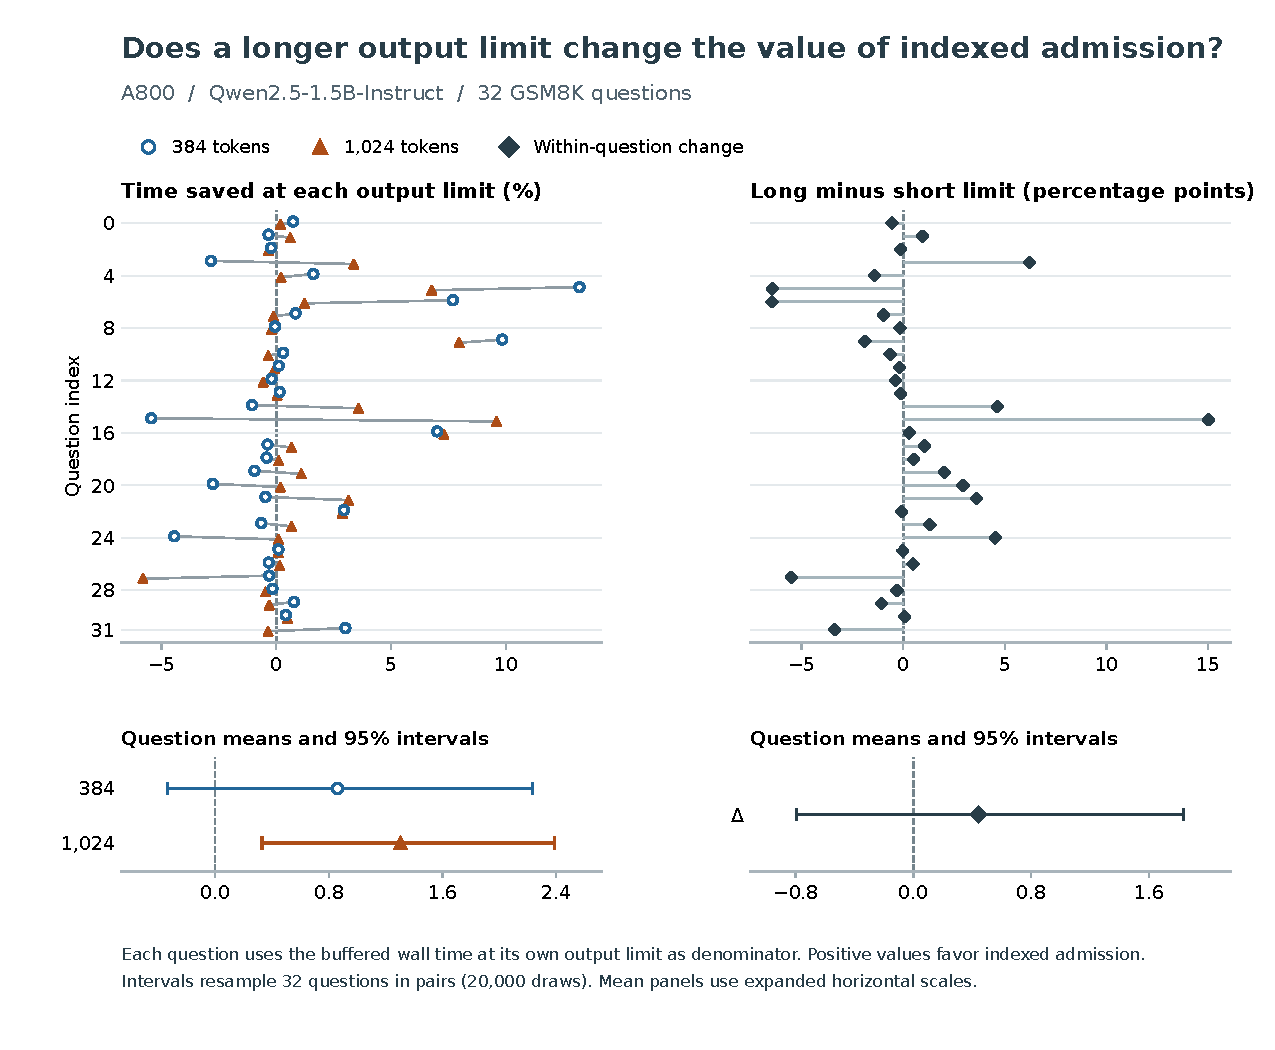
\includegraphics[width=.97\textwidth]{cap-comparison.pdf}
\caption{Per-question savings in synchronized A800 wall time. Each observation compares the indexed and buffered gates under one output limit. The right-hand contrast subtracts the short-cap saving from the long-cap saving on that question. The lower panels show question means and paired 95\% bootstrap intervals on expanded axes.}\label{fig:cap}
\end{figure}
\section{Two comparisons with classical scheduling}\label{app:precedence}
First consider a fixed prerequisite set on the original jobs. A job becomes eligible once every job in its prerequisite set has finished. Set $(N,P,Q,B)=(9,5,9,0)$. Start job 1 at time zero with work 10. Give jobs 2 through 5 works $(4,3,2,1)$ and votes $(A,A,B,B)$, respectively. No vote has been revealed when the initial allowance of five starts is established. For job $i=2,\ldots,5$ use start time $5-w_i-1/4$ if it should have finished at time 5 and $5-w_i+1/4$ otherwise. These starts preserve index order and obey the gate. At time 5 all three histories considered below have five starts, two completions and two idle slots.

With completed set $\{2,4\}$ or $\{3,5\}$, the two known votes disagree. A five-vote prefix can then lead by at most three, leaving four outstanding votes, so a sixth start is safe. With completed set $\{2,3\}$ both votes favor $A$. Five initial $A$ votes remain possible and would lock the decision, which makes the sixth start unsafe. The earliest compatible serial stops are $6,6,5$, respectively. The two permitting sets have empty intersection. A fixed prerequisite set on the original jobs would have to be empty to allow both, and would incorrectly allow the third history. An external capacity depending only on time cannot distinguish these three states either. General encodings with auxiliary jobs or logical predicates can represent additional dependencies.

A separate example isolates the role of the occupancy comparison. Let four unit jobs run on three slots in index order. Jobs 3 and 4 require job 1 to finish. Immediate refill runs jobs 1 and 2 and then jobs 3 and 4, with two units of virtual time at width two. Another policy starts job 1 at zero, jobs 2 and 3 at one and job 4 at $1.5$. It spends $1.5$ units at width one, $0.5$ at two and $0.5$ at three. The concave prices $(c_1,c_2,c_3)=(1,2,2.5)$ give physical costs $4$ and $3.75$, respectively. Greedy starts and finishes every job by the time its competitor does in virtual time. This property alone permits higher physical cost even on a concave clock. The zero-allowance voting gate adds the nonincreasing bound on active width used in Appendix~\ref{app:major}.

\section{Prospective clock validation and the frequency of useful delays}\label{app:transfer}
We froze the protocol, driver and four trial orders before starting the A800 experiment. vLLM 0.8.5 V0 ran the BF16 Qwen2.5-1.5B-Instruct checkpoint with a 512-token input, prefix caching and chunked prefill disabled, and fixed generation lengths. Calibration and validation used separate engine processes in the same device session. After warmup, eight randomized calibration blocks each measured 96 cached decode steps at three widths after a 64-step prelude. We took the median of the eight window means at each width, wrote both contrasts and their decision classes, and verified a local copy of the prediction before launching validation. Against immediate admission, the staged policy waits until a request finishes before launching the last request. Both arms use the same inputs and generate the same number of tokens.

Each of 12 validation blocks measured all four arms in balanced orders. We timed the whole panel from before the first submission to a drained engine after a device synchronization. For a directional prediction at least one percentage point from zero, the prespecified interval had to lie strictly on the predicted side of zero, and the observed median had to be within two percentage points of the prediction. For a smaller prediction we required the interval to lie inside $[-2,2]$ percent and the same tolerance on the median. Both comparisons had to pass. We report the third and tenth ordered paired effects. Under independent blocks with a common continuous median, this interval has 96.14\% coverage. Session drift could affect that interpretation. Output token fingerprints agreed in every measured pair.

\begin{figure}[htbp]\centering
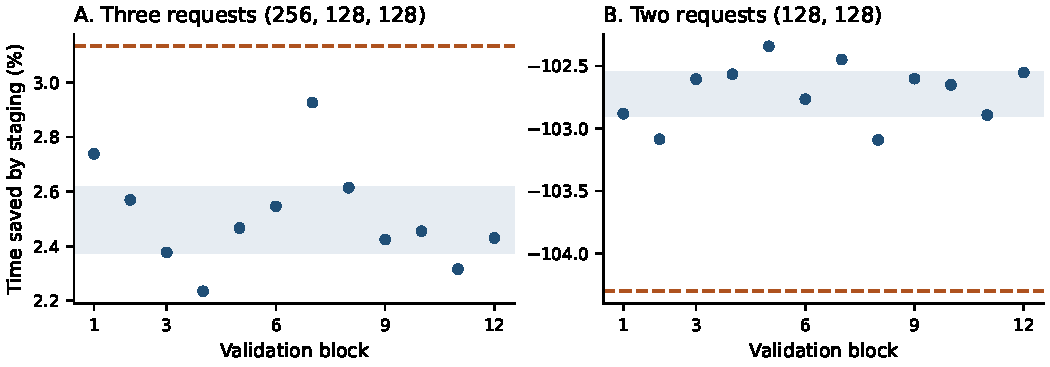
\includegraphics[width=.83\textwidth]{transfer-blocks.pdf}
\caption{Time saved by staging, relative to concurrent admission. Points show the 12 paired wall measurements. The dashed lines give the predictions sealed before validation. Shading spans the third to tenth ordered effects. Each panel uses its own vertical scale. Negative values indicate that waiting increased whole-panel time.}\label{fig:transfer}
\end{figure}

In the three-request test, the arm medians were 1,234 and 1,203 ms. For the two-request control they were 602 and 1,221 ms. Averaging the three-request paired changes allows an additive accounting of the 2.508 percentage points saved. Engine steps returning only cached tokens contributed $+3.165$ points, steps returning a first token contributed $-0.644$, and the remaining host time contributed $-0.013$. Per-step host timing includes engine work beyond kernels. The comparison does not measure waiting time in a multi-tenant queue.

We separately replayed both actions on the first three paths in original order from each of the 200 archived GSM8K questions. The rule was fixed before computing this retrospective analysis. The lengths came from Qwen3-4B-Base, including three paths that reached the 31,744-token cap. Times use the Qwen2.5 three-width clock throughout. Staging helped 66 of 200 panels and increased question-average time by 26.73\% when applied throughout. Even with advance knowledge of the three realized lengths, choosing the faster of these two actions could save only 0.364\% on average (0.205\% by summed times) relative to immediate admission. This calculation concerns three-path prefixes of one archive and exactly two actions. Serving traffic, other actions, and other operating clocks can give different opportunity rates.

\paragraph{What a call guarantee changes.}
In the same archive we also allowed the complete 16-path vote ($N=Q=16$) and checked the full-panel winner of every policy on every question. A synchronous four-sample batch exceeded the serial stopping point by at least two starts on 98 of 200 questions. A four-slot eager scheduler using only the absolute limit did so on 148. Enforcing $B=1$ prevented all such overruns and saved 1.56 starts per question compared with that eager policy, at a 35.36\% increase in question-average modeled time under the DeepSeek 3,968-token clock. A two-sample barrier already respects $B=1$. A deployment needs to value the additional per-question protection enough to justify its latency cost.

\section{Collecting a specified number of verified candidates}\label{app:rpass}
Consider $N$ ordered, irrevocable candidates on the same shared clock. Candidate $i$ reveals a binary verification result after positive work $w_i$. Serial execution stops at its $r$th pass, or at exhaustion of all $N$ candidates, for $1\le r\le N$. Let $K$ denote this stopping index. A policy may start at most $K$ candidates on every compatible completion of its observations. It returns once it observes $r$ passes or completes all $N$. As in voting, work and verifier outcomes are fixed within each comparison.

\begin{proposition}
On any reachable nonterminal history with $s$ observed passes and $f$ failures, the exact cumulative launch frontier is
\[
       \min\{N,s+f+P,r+f\}.
\]
Immediate refill obeys the occupancy comparison \eqref{eq:major} for this task. For fixed slot count $P$, taking the worst case over $N,r$, works and outcomes gives the same exact price ratio $\max_j\widehat c_j/c_j$. The ratio can be attained with finite integer work.
\end{proposition}
\begin{proof}
Initially $J=0\le\min(N,r+f)$, where $J$ is the number launched. Suppose this invariant holds. All observed failures lie in the first $J$ positions. A compatible continuation cannot have stopped before $J$ by the zero-overrun promise on prior starts. From $J$ onward no prefix shorter than $r+f$ can contain $r$ passes. Making all unseen candidates pass attains $\min(N,r+f)$, including when fewer than $r$ passes are possible. The slot cap supplies the other term in the frontier. New failures only increase the cumulative limit. On return with $s=r$, the frontier implies $J\le r+f=s+f\le J$, so all starts have finished. Their indices form the serial stopping prefix by the guarantee. Exhaustion also completes exactly the serial prefix. Thus every admissible schedule performs the same work on a given input.

Greedy's permitted active width $\min(P,N-s-f,r-s)$ cannot increase when more jobs finish. The cumulative frontier is nondecreasing. These properties give the shortened-input comparison and the time compression proof of Appendix~\ref{app:major} with the same jobwise inclusions. The concave-majorant argument then gives the upper ratio.

For sharpness, take a hull chord with endpoints $a<j<b$ attaining the maximum at $j$. Set $r=b$. All candidates fail. Take $a$ long initial jobs of length $L=S/(j-a)$ and $S$ unit jobs where $S=\mathrm{lcm}(b-a,j-a)$. Here $N=a+S\ge b$. With a continuing supply of unit jobs greedy fills to $b$, whereas a policy capped at $j$ fills to $j$. Greedy spends $S/(b-a)$ units of virtual time at width $b$ and the remainder of $L$ at width $a$, counting virtual padding with $c_0=0$ if $a=0$. The comparator spends all $L$ units at width $j$. The time ratio is $\widehat c_j/c_j$. When the maximum is one, a single candidate attains it. No inference about deployed verification policies is required for this corollary.
\end{proof}
